\section{Introduction}
Healthcare pathways are critical for reducing clinical variability, affecting operational excellence, and maximizing health outcomes \cite{Lin2001}. They define the execution sequence of clinical activities as patients move through a treatment process, a department, a hospital, or a wider health organization %(e.g., a District Health Board) 
\cite{Huang2016}. The accurate definition of healthcare pathways and patient conformance to those pathways is an issue of increasing relevance as precision medicine enables targeted approaches and diagnostic splitting. The proliferation of pathway branches is exponential, and pathways are increasingly non-linear. 

Most healthcare pathways result from clinician-led practice rather than explicit pathway design via a consensus model and systems approach. In addition, healthcare pathways “shift” dynamically as steps in the pathway are altered or resources change along the pathway. If no explicit redesign of pathways is performed, then the providers of the pathways (and its associated resources) may be unaware of the change \cite{Zhang2015}. Pathway discovery (identification of pathways without a priori knowledge), conformance analysis (including gaps in care and clinical variability) and pathway enrichment (enrichment of a priori models with additional event data) are critical for healthcare services now, and into the future \cite{Baker2017}.

Past studies have shown that there is potential for informative healthcare pathways to be extracted from hospital health records \cite{Xu2017}, \cite{Iwata2013}, but there is currently no consensus on a systematic healthcare pathway mining method that supports explicit design and conformance analysis of concise and comprehensible healthcare pathway models. The research described in this paper investigates the utilization of Business Process Modelling (BPM) as outlined by Becker et al. \cite{Becker2000} to provide a scaffold for healthcare pathway discovery, conformance analysis and enrichment. The main objectives of applying BPM to healthcare data include:
\begin{enumerate}
    \item Pathway discovery
    \begin{itemize}
        \item Investigate the potential of ProM (a process-mining software package) to discover healthcare pathways from hospital records \cite{VanDongen2005}.
    \end{itemize}
    \item Conformance analysis
    \begin{itemize}
        \item Apply BPM conformance analysis to discovered healthcare pathways. 
        \item Improve detection of possible non-conformance and explain anomalies.
    \end{itemize}
    \item Data enrichment
    \begin{itemize}
        \item Investigate correlation between healthcare pathway and performance-determining factors (e.g., patient length-of-stay, readmission rate).
    \end{itemize}
\end{enumerate}

\section{Healthcare Pathway Mining Methodology}
This chapter outlines the proposed process mining pipeline designed for mining healthcare pathways from hospital records using business process modelling tools. This study adopts the scientific computing practices recommended by Wilson et al. \cite{Wilson2014}, \cite{Wilson2017} to ensure that all results are reproducible. The proposed process mining pipeline consists of three major sections that correspond to each of the three main objectives (i.e. pathway discovery, conformance, and enrichment). An overview of the process mining pipeline designed for this study is shown in Fig.~\ref{fig:pipeline}. It comprises three phases, which are pathway discovery, conformance analysis, and data enrichment. The following sections elaborate these phases and their respective objectives.

\begin{figure}[t]
\centering
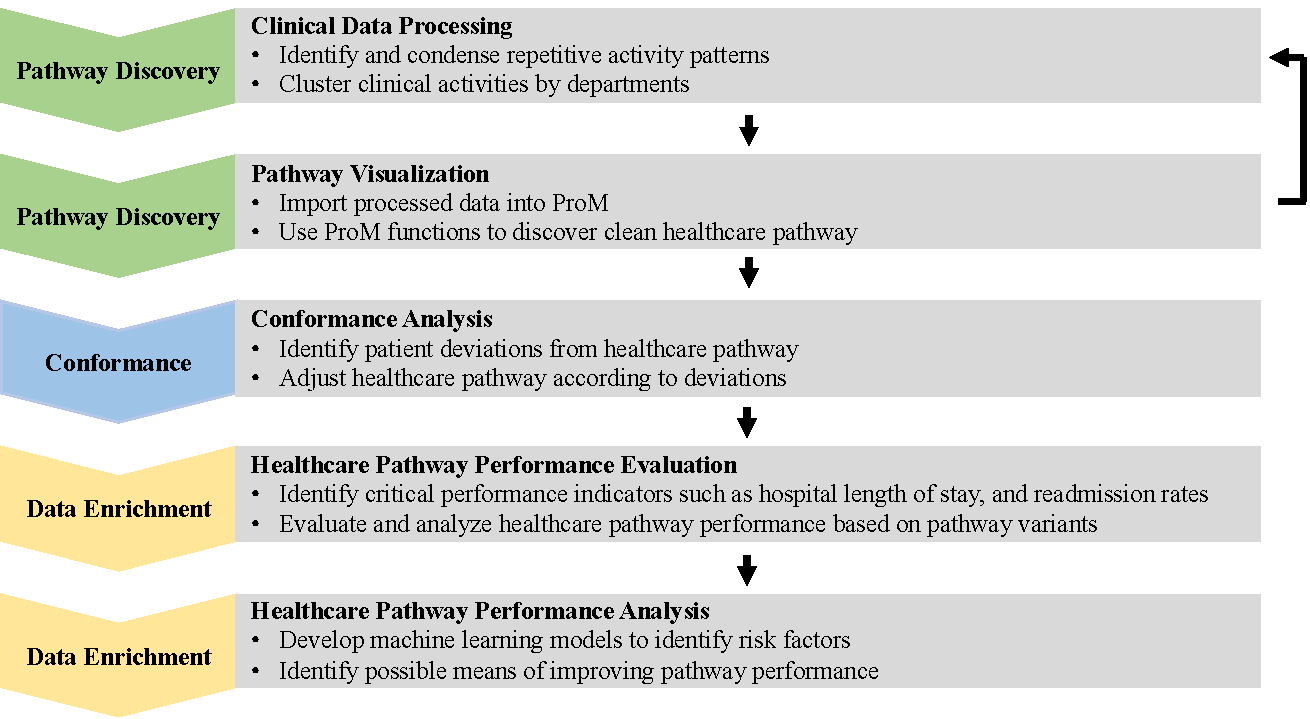
\includegraphics[width=\textwidth]{images/pipeline_diagram_journal.pdf}
\caption{The process mining pipeline comprises three sections, which
  are subdivided into five steps: Clinical data processing, pathway
  visualization, conformance analysis, healthcare pathway conformance
  evaluation, and prescriptive analytics of healthcare pathways. The
  first three steps are connected in two iterative cycles.}
\label{fig:pipeline}
\end{figure}

This study evaluates ProM (version 6.7) as the main process mining tool\footnote{\url{http://www.promtools.org}}. 
ProM is an open-source process mining software that is effective for construction of business models from input data files. The use of ProM in the healthcare sector has not been thoroughly explored in the past, but Van Der Aalst et al.  have demonstrated the applicability of the software for industrial processes \cite{VanDerAalst2007}. ProM is chosen for this study because it has an intuitive user interface and supports many process mining plug-ins \cite{VanDongen2005}. The process mining and conformance analysis plug-ins supported by ProM are well documented. All these features of ProM make it easy for the process mining steps in the pipeline (see Fig.~\ref{fig:pipeline}) to be repeated by users with no background in process mining.

\subsection{Healthcare Pathway Discovery}
Healthcare pathway discovery is the first phase of the proposed process mining pipeline. It consists of two steps: clinical data processing and pathway visualization, which are conducted iteratively until a concise model is produced.
The aim is to use patient healthcare records stored in hospitals’ information systems to design a concise pathway model that is easy for clinical interpretation. Therefore, clinical input is critical to the selection of appropriate processing methods. 

%\subsubsection{Clinical Data Processing}
 A pathway model is a set of pathway variants. Each pathway variant is
 a unique activity sequence of a complete patient trace. The ProM
 plug-in \plugin{Explore Event Log} extracts pathway variants from patient traces, and the total number of pathway variants is an indicator of the level of clinical variation between patient traces. 
 
However, healthcare pathways generally have much higher levels of complexity than standard business processes, and unprocessed clinical data contains too many clinical variations for a clean and concise pathway model to be mined \cite{Huang2013, Veiga2010}.
In order to reduce healthcare pathway variations to a meaningful pathway model, the pathway variants visualized by the plug-in \plugin{Explore Event Log} are examined closely to determine the most suitable processing methods. 
There are three effective methods for reducing clinical variations without filtering patient traces:

\begin{description}
    \item[Cluster clinical activities] that are similar in nature so that the range of activities is reduced to a manageable size, e.g., `Abdomen CT scan' and `Pelvis CT scan' could be clustered into a single activity under `CT scan'.
    \item[Merge consecutive clinical activities] that are performed consecutively into a single activity, e.g., a patient receiving the same medication five times on the same day could be regarded as a single activity.
    \item[Condense repetitive activity patterns] 
         that repeat but exhibit variable cycle length. These patterns indicate an activity that must be performed periodically while the patient is waiting for a different activity to begin, e.g., lab tests to monitor a patient’s condition, medication to prevent infection. These repetitive patterns could be condensed into a single, parallel activity.
\end{description}
Clinical input is highly recommended at this step particularly for complex or unfamiliar healthcare pathways. 

%\subsubsection{Pathway Visualization}

\subsection{Healthcare Pathway Conformance Analysis}
Conformance analysis evaluates the degree to which a healthcare pathway model captures movement of patient traces by comparing the pathway model to clinical data. 
Accuracy of the discovered healthcare pathway model is validated if the majority of the patient traces conform to the model. Patient traces rarely all follow identical pathways, so the healthcare pathway model is not expected to capture all patient traces. The objective is to discover a healthcare pathway model that captures the fundamental structure of most patient traces. 

ProM offers tools for conformance analysis of healthcare
pathway models: Its plug-in \plugin{Inductive Visual Miner} compares
patient traces from input clinical data to a healthcare pathway model
and indicates patient traces, which are deviating from the pathway
model.
For this purpose, the pathway model is visualized as process tree,
which is a hierarchical map comprised of decision nodes and
tasks representing clinical activities
\cite{25a7fd818bf44606a903d9b78b95cdd3}.
Therefore, process trees enable the identification of pathway branches
throughout the healthcare pathway model (c.f. Sec~\ref{Sec:DiscoveryConformance}).

If valid patient traces deviate from a healthcare pathway model, 
adjustments are made to the model to improve patient conformance.
A typical example might be the introduction of a new form of
treatment, which has not been included into the model, yet.
Including these findings into the model leads to an iterative approach
between pathway discovery and conformance analysis (Fig.~\ref{fig:pipeline}).
Conversely, if patient traces do not conform to a healthcare pathway
model, conformance analysis can identify where these invalid
patient traces deviate from the model and investigate the reason for
the discrepancy, e.g., clinicians following obsolete pathways or data errors.

\subsection{Healthcare Pathway Data Enrichment}
% \subsubsection{Healthcare Pathway Performance Evaluation}
Data enrichment of healthcare pathways is the third phase of the
discussed process mining pipeline (Fig.~\ref{fig:pipeline}).
It comprises two steps: Healthcare pathway performance evaluation and
healthcare pathway performance analysis.

The main objectives of evaluating healthcare pathway performance are
to understand the strengths and weaknesses of the current pathway design,
and to identify potential methods of improvement. Possible indicators
of healthcare pathway performance include waiting times of clinical
activities, hospital length of stay, recovery time and readmission
rates \cite{Rotter2008_pathways}.
Most of these indicators can be calculated or estimated using standard clinical timestamps.
For surgical healthcare pathways, Postoperative Length of Stay (PLS)
is one of the critical indicators for evaluating healthcare pathway
performance \cite{Pearson2001_pathways}.

Analysing the performance of healthcare pathways with respect to
pathway variants and other possible influencing factors like
demographics or patient specific pathway characteristics, e.g. length
of Surgery (LoS), is the final step of the process mining pipeline
(Fig.~\ref{fig:pipeline}).
Due to the fact, that most pathway performance indicators do not
follow normal distributions, while exhibiting significant stochastic
volatility, neither classical hypotheses tests \cite{Goodman2008_p-value}, nor point-predicting
machine learning models are appropriate for analysing healthcare
pathways.
Instead, probabilistic machine learning models
\cite{Ghahramani2015_PML} are used for extracting interpretable models
from healtcare pathways (Sec.~\ref{sec:ML}).
For this purpose, feature engineering \cite{DongLiu2018_FE} from
the patients's pathway traces (e.g. LoS, pathway variant),
demographics (e.g. age), as well as medical documentation like written
diagnosis, time series, or images becomes important.
In order to demonstrate this approach, the following case study
discusses a probabilistic machine learning model for PLS, which
takes into account pathway variants
(Sec.~\ref{Sec:DiscoveryConformance}), as well as demographics, and
LoS (Sec.~\ref{sec:ML}).

\section{Case Study: Appendicitis Healthcare Pathways}
This section discusses the healthcare pathway discovery process for an
appendicitis case study. For this purpose, two years’ worth of data
from 2015 to 2017 from 415 appendicitis patients (201 female, 213
male) %DS19fA0
have been analysed. 
A second case study on 52 cholecystitis patients is presented in \ref{sec:Cholecystitis}.
The patients' traces from both case studies were collected from North Shore Hospital in Auckland, New Zealand.

\subsection{Appendicitis Pathway Discovery and Conformance Analysis}
\label{Sec:DiscoveryConformance}
The appendicitis pathway model, which has been generated by ProM's
plugin \plugin{Explore Event Log}, is shown in
Fig.~\ref{fig:appendicitis pathway variants} in form of a pathway
variant plot.
The pathway variants are extracted without activities related to medication (i.e. preoperative and postoperative cefuroxime/metronidazole) because the clinicians confirmed that antibiotics are usually taken while the patient is waiting for surgery or discharge. The duration of these activities are therefore highly variable and result in a high number of unique pathway variants.

%The variant specific numbers of patient traces given in  Fig.~\ref{fig:appendicitis pathway variants} are repeated in Tab.~\ref{table:appendicitis variant table}.
The pathway variant plot visualizes the 13 pathway variants of the
appendicitis model sorted from the most common pathway (index 0) to
the least common pathway (index 12).
The top four variants account for approximately 88\% of the patient
traces (Tab.~\ref{table:appendicitis variant table}).
All clinical activities are represented by a start event and a stop
event.
The activities are colour coded such that the same colour refers to the same clinical activity. The most frequent pathway variant (index 0) only consists of anesthesia and surgery, while the second most frequent variant (index 1) also includes preoperative X-ray.
The pathway variant indices are used in Sec.~\ref{sec:ML} as one-hot
encoded feature of the probabilistic machine learning model.

\begin{figure}[t]
\hspace{-2cm}
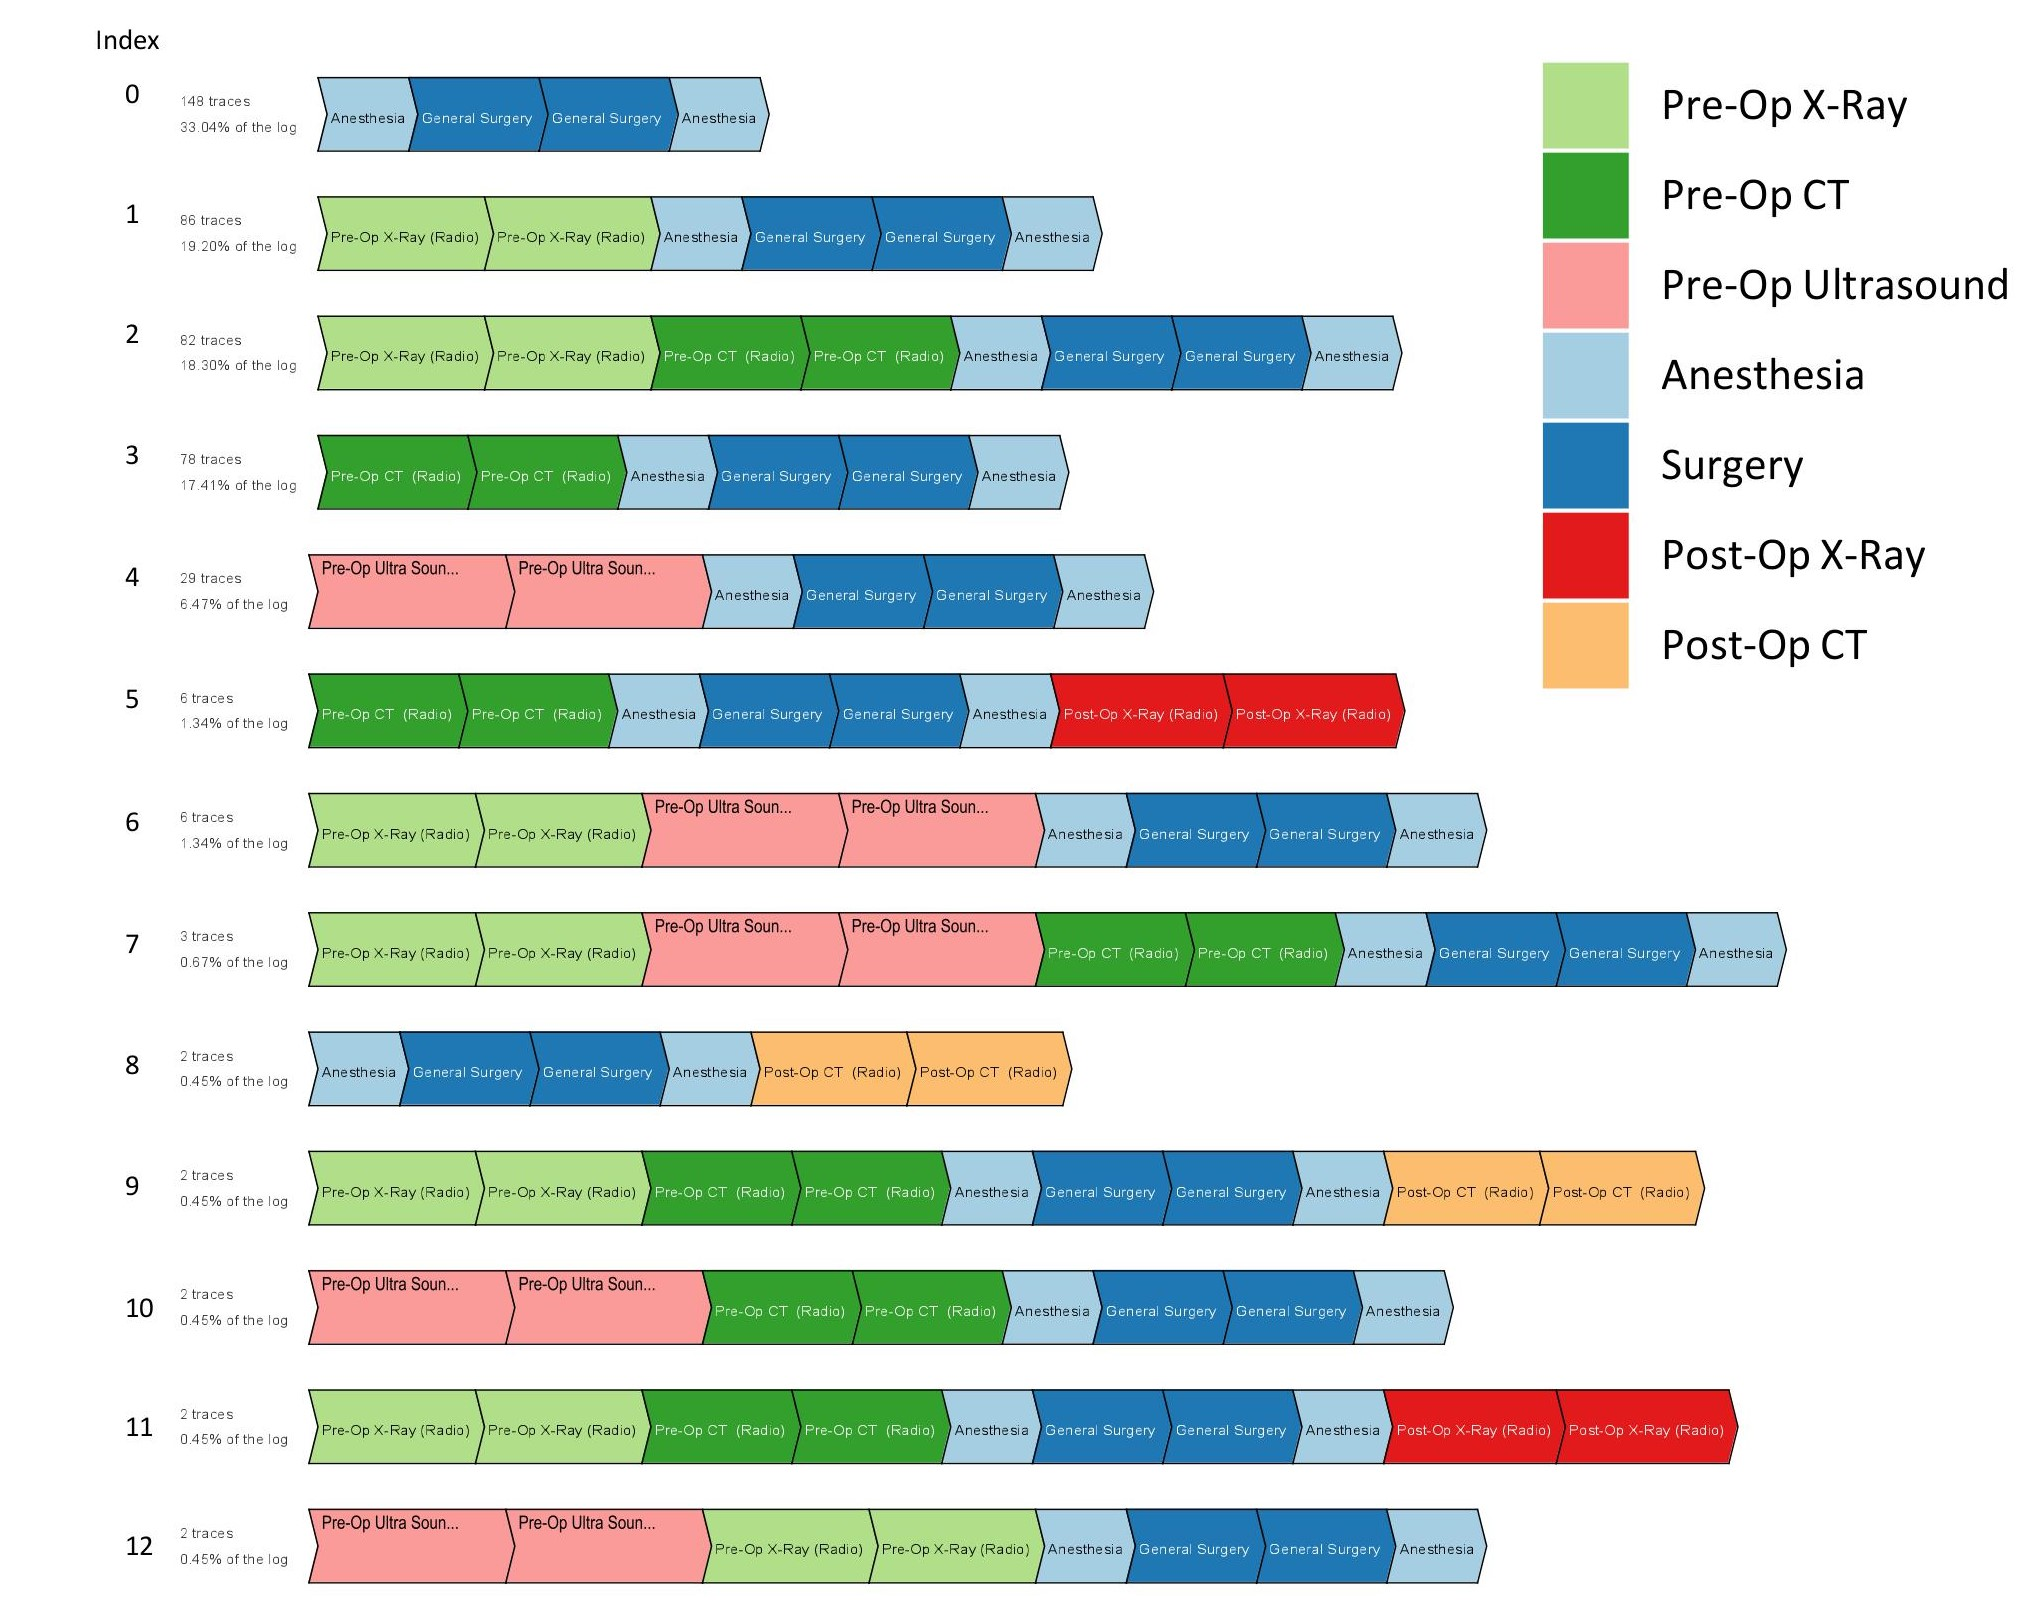
\includegraphics[width=1.5\textwidth]{images/appendicitis_variant_index_anes.jpg}
\caption{Appendicitis pathway variant plot auto-generated by ProM's
  plugin \plugin{Explore Event Log}. 
  For the purpose of readability the legend was added and the
  statistics on the left are repeated in Tab.~\ref{table:appendicitis variant table}.
 The top four variants account for approximately 88\% of the patient
 traces. They are modelled as one-hot encoded features V0, V1, V2, and V3
 in Sec.~\ref{sec:ML}, while pathway variants V4--V12 together represent
 the base model.
 }
\label{fig:appendicitis pathway variants}
\end{figure}
\clearpage

\begin{table}[t]
\centering
\caption{Number of patient traces shown in Fig.~\ref{fig:appendicitis pathway variants} that follow each appendicitis pathway variant.}
\label{table:appendicitis variant table}
\begin{tabular}{ r c c }
 \hline
 \hline
 Variant & Number of patients & Percentage \\ 
 \hline
 0 & 148 & 33.04\\ 
 1 & 86 & 19.20\\ 
 2 & 82 & 18.30\\ 
 3 & 78 & 17.41\\ 
 4 & 29 & 6.47\\ 
 5 & 6 & 1.34\\
 6 & 6 & 1.34\\ 
 7 & 3 & 0.67\\ 
 8 & 2 & 0.45\\ 
 9 & 2 & 0.45\\ 
 10 & 2 & 0.45\\ 
 11 & 2 & 0.45\\ 
 12 & 2 & 0.45\\ 
 \hline
 \hline
\end{tabular}
\end{table}


The first stage of the appendicitis pathway model visualized by \plugin{Inductive Visual Miner} from processed clinical data is shown in Fig.~\ref{fig:ivm pathway model example}. Unlike the pathway variants, the appendicitis pathway model incorporates activities representing antibiotics. The model indicates that 42 patients perform ultrasound and 183 patients perform X-ray upon admission. 

\begin{figure}[t]
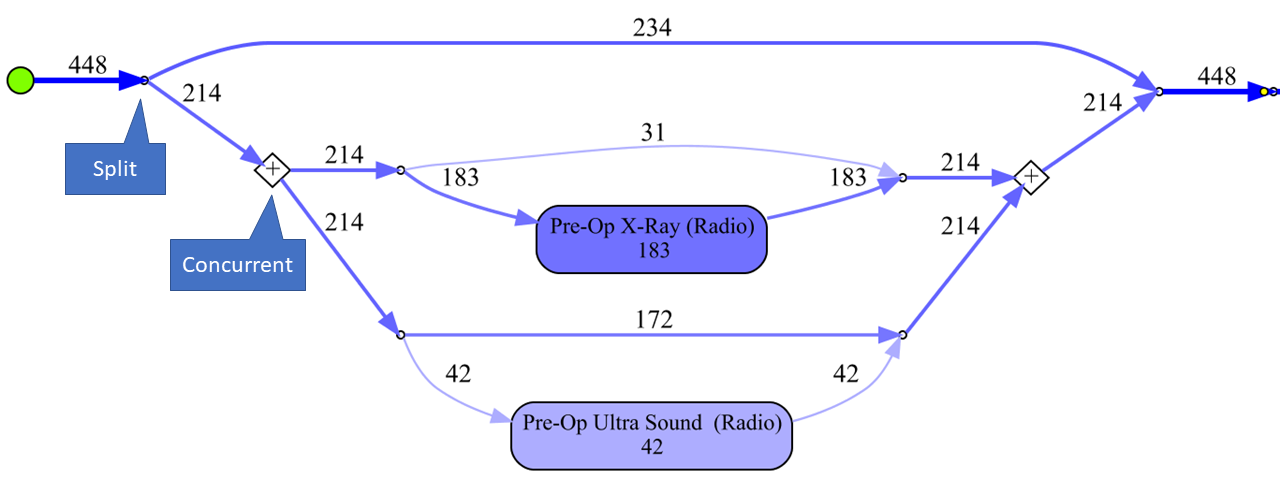
\includegraphics[width=\textwidth]{images/ivm_appendicitis_first_stage_example.png}
\caption{First stage of the appendicitis pathway model generated by
  ProM. There are 214 patients that enter the first stage of the
  treatment pathway, which consists of X-ray, or ultrasound, or both.
  Please refer to Leeman's manual on \plugin{Inductive Visual Miner} for details on the model notations used in  Fig.~\ref{fig:ivm pathway model example} \cite{leemansinductive}.}
\label{fig:ivm pathway model example}

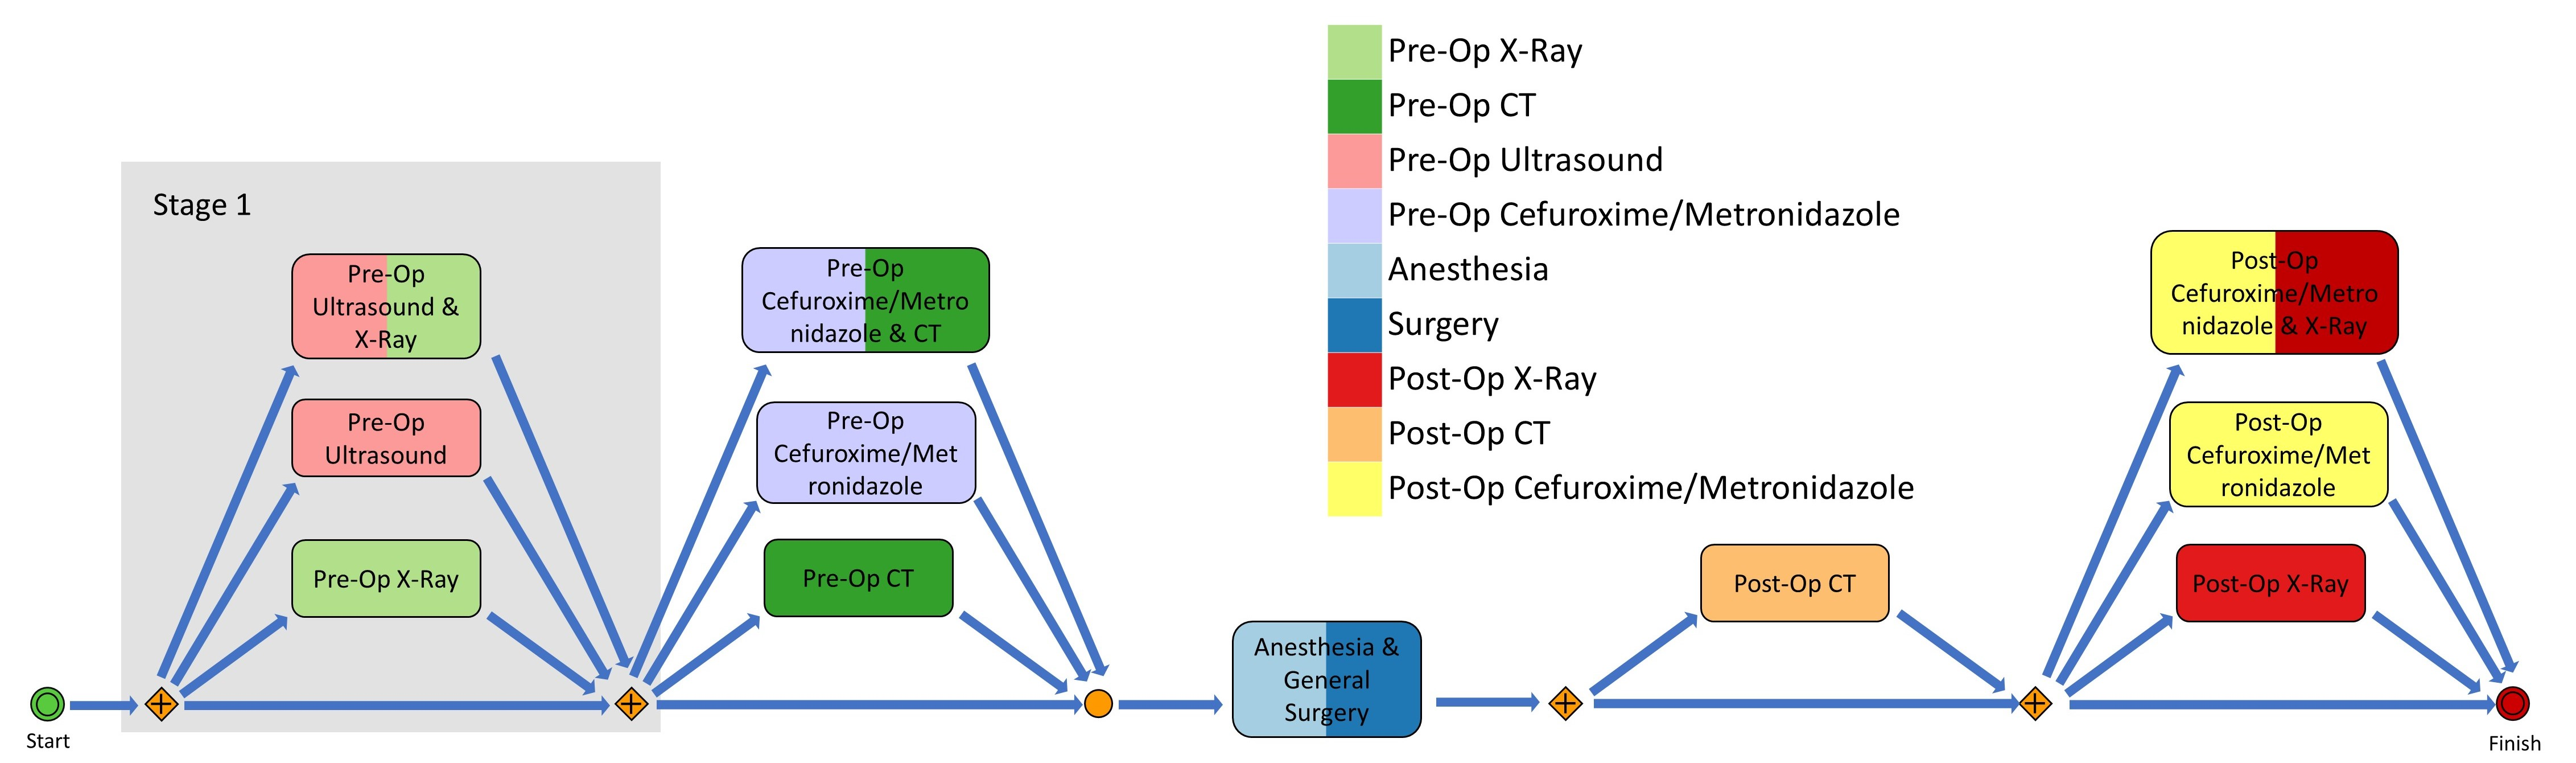
\includegraphics[width=\textwidth]{images/communicative_appendicitis_process_models_anes.jpg}
\caption{Appendicitis pathway model. All pre-operation and post-operation activities belong to radiology and pharmacy departments. Pre-operation antibiotics are taken in the second stage of the treatment pathway.}
\label{fig:appendicitis pathway model}
\end{figure}

The ProM notations for pathway models are complex and optimal for detailed analysis, so the appendicitis pathway model discovered by ProM is reformulated under new notations for easy clinical interpretation. The new model notations are summarized in Table \ref{table:notation table}, and the reformulated appendicitis pathway model is shown in Fig.~\ref{fig:appendicitis pathway model}. The section of the model labelled as `Stage 1' in Fig.~\ref{fig:appendicitis pathway model} corresponds to the same section shown in Fig.~\ref{fig:ivm pathway model example}. This is the final pathway model that has been compiled based on clinical input to account for valid patient deviations, and all patient traces conform to the updated pathway. The most frequent pathway variant (index 0) shown in Fig.~\ref{fig:appendicitis pathway variants} corresponds to the horizontal path from start to finish in Fig.~\ref{fig:appendicitis pathway model}.

\begin{table}[t]
\centering
\caption{Definitions of new pathway model notations.}
\label{table:notation table}
\begin{tabular}{ l c l }
 \hline
 Notation & Symbol & Definition \\ 
 \hline
 Orange Diamond 
 &
%\raisebox{-\totalheight}{\includegraphics[width=0.3\textwidth, height=60mm]{images/myLboro.png}}
 \raisebox{-3pt}{
\includegraphics[width=0.5cm]{images/decision_node.png}}
 & Decision Point, indicating exclusive choice \\ 
 \hline
 Orange Connector 
 & 
 \raisebox{-3pt}{
\includegraphics[width=0.5cm]{images/connection_node.png}}
 & Pathway Connection Point \\
 \hline
 Green Connector 
 & 
 \raisebox{-3pt}{
\includegraphics[width=0.5cm]{images/start_node.png}}
 & Starting Point \\
 \hline
 Red Connector 
 & 
 \raisebox{-3pt}{
\includegraphics[width=0.5cm]{images/finish_node.png}} 
 & Finishing Point \\
 \hline
\end{tabular}
\end{table}

%\include{appendicitis_length_of_stay}

\subsection{Data Enrichment of Appendicitis Pathways}
\label{sec:ML}
The following section investigates the question if the pathway variants of the appendicitis case study are relevant exogenous variables for predicting PLS.
This is quite a challenging task, because the individual healing process is expected to depend on personal factors like age \cite{polanczyk2001impact} as well as the individual severity of the appendicitis inflamation, which in general is unknown at this stage of the data analysis, but might be captured by proxis like Length of Surgery (LOS).

For the purpose of this analysis, the patient's $PLS_i$, which is given as time interval between end of surgery and discharge, is converted into number of days after surgery. Therefore, a $PLS$ of one corresponds to a patient, who has been discharged the day after the surgery. However, we've found that 3 of the $N=448$ patient traces had a PLS of zero, because the surgery ended shortly after midnight and the patients were discharged on the same day. In order to simplify our analysis, the interpretation of PLS was broadend to /number of night rests/ after surgery, such that the PLS of these three patients could be casted to one.

Analysing the PLS of the 448 appendicitis patients reveals a histogram, which closely resembles a Geometric distribution
\begin{equation}
Pr(PLS=k) = \text{Geom}(p) = (1-p)^{k-1}p^{k},
\end{equation}
which is parametrized by probability $p$ of being discharged at the $k^\text{th}$ day respectively $k$ night rests after surgery. 
However, estimating $p$ as inverse mean of the observed PLS to 
\begin{equation}
 \hat{p} = \frac{N}{\sum\limits_{i=1}^N PLS_i} \approx 61.8\%	
\end{equation}
reveals that the average discharge probability $\hat{p}$ does not generalize well over the cohord, because the number of patients being discharged at the first day after surgery is underestimated and the number of patients being discharged at second and third day after surgery is overestimated (Fig.~\ref{fig:Geom}).

\begin{figure}
    \centering
    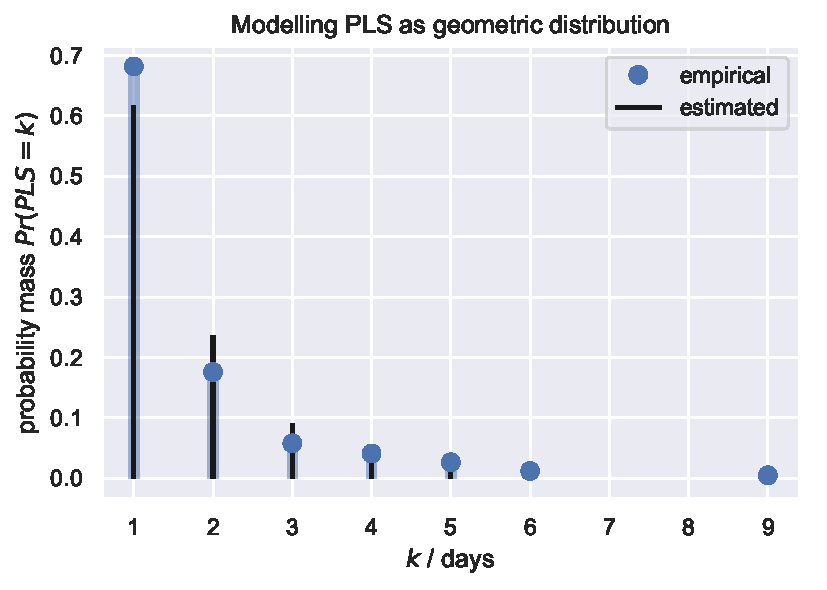
\includegraphics{images/DS19eH1_G0__empirical_geometric.pdf}
    \caption{Caption}
    \label{fig:Geom}
\end{figure}

Following a probabilistic programming methodology the individualized discharge probability $p_i = p_i(x_i)$ is modelled as generalized linear model (GLM) using the inverse logistic function (logit) as link function and the Geometric distribution for generating the likelihood. 
For the following analysis, we are comparing two different models of discharge probability $p_i$ with $x_i = (LOS_i, \text{log}(age_i), V_{0,i}, V_{1, i}, V_{2, i}, V_{3, i})$: 
\begin{eqnarray}
\label{modelA}\text{model A}&:& \text{logit}(p_i) \sim LOS_i + \text{log}(age_i) \times (V_{0,i} + V_{1,i} + V_{2,i} + V_{3,i}),\\
\label{modelB}\text{model B}&:& \text{logit}(p_i) \sim LOS_i + \text{log}(age_i) \times (V_{0,i} + V_{1,i}) + V_{2,i} + V_{3,i}. 
\end{eqnarray}
These two models have been selected because they were the most credible ones based on WAIC and LOO statistics. The explanatory variables $V_{j}$ are categorical with 
\begin{equation}
V_{j,i} = \begin{cases}
	1: & V_{j,i} = j,\\
        0: & \text{otherwise}.
\end{cases}
\end{equation}
Therefore, the case $V_{0,i}=V_{1,i}=V_{2,i}=V_{3,i}=0$ corresponds to variants V4--V12 of Fig.~\ref{}.
These models make the simplifying assumption that the individualised probability of discharge $Pr(PLS_i=k|x_i)$ can be estimated from the information $x_i$ being available at the end of surgery, when future treatment steps and therefore the complete pathway variant for the respective $i^\text{th}$ patient have been decided on:
\begin{equation}
\begin{split}
Pr(PLS_i=k|x_i) & = \text{Geom}(p_i|x_i) \\
                  & = (1-p_i)^{k-1}p_i^{k} \\
          %        & = \left(1-\text{logistic}(f(x_i))\right)^{k-1}\text{logistic}(f(x_i))^{k} \\
          %        & = \left(1+e^{f(x_i)}\right) \left(2 + e^{-f(x_i)} + e^{f(x_i)}\right)^{-k}
\end{split}
\end{equation}
with $p_i$ being modelled either by Eqn. \eqref{modelA} or \eqref{modelB}.

The statistical model has been fitted using PyMC3 \citep{Salvatier2016_PyMC3} version 0.24.2 using the No-U-Turn Sampler (NUTS) with 20,000 samples, 2,000 tuning steps, 2 chains, and an acceptance rate 90\%. The 95\% credible intervals of the estimated model coefficients are shown in Fig.~\ref{fig:forest_plots}. The Gelman-Rubin convergence statistic R-hat is close to one for all coefficients. 
However, for Model A the coefficients of the interaction terms $\text{log}(age_i)\times V_2$ and $\text{log}(age_i)\times V_3$ are close to zero with negative expectation values but a 25\% and 15\% probability of being larger than zero. 
Therefore, we have decided to focus the following analysis of the fitted model on Eq.~\ref{modelB} for which all credible intervals exclude zero (Fig.~\ref{fig:forest_plots}b).

\begin{figure}
    \centering
    \begin{tabular}{ll}
(a) Model A \eqref{modelA} & (b) Model B \eqref{modelB}\\
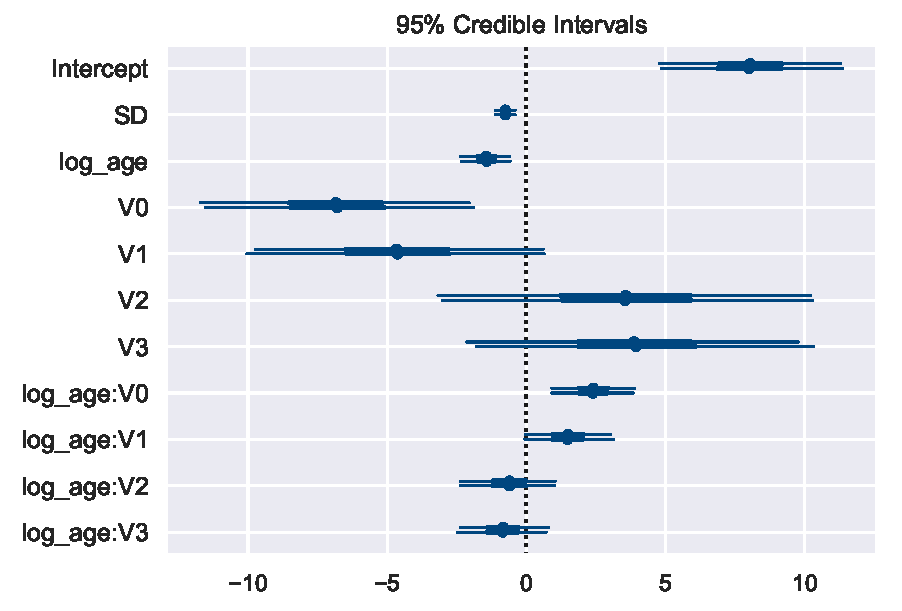
\includegraphics[width=0.5\textwidth]{images/DS19fm0_c0__forestplot_model_A.pdf}&
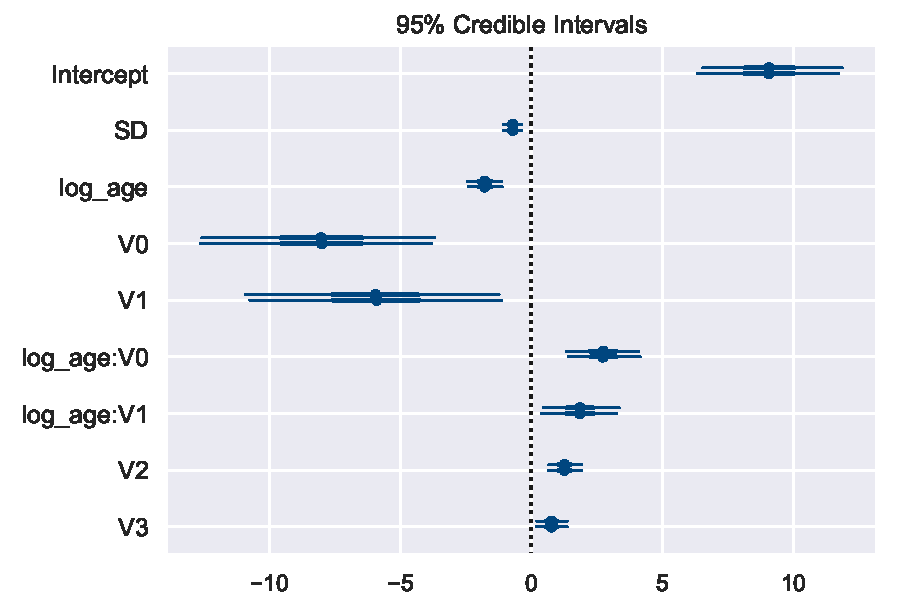
\includegraphics[width=0.5\textwidth]{images/DS19fk1_c0__forestplot_model_B}\\
\end{tabular}
    \caption{Caption}
    \label{fig:forest_plots}
\end{figure}

The estimated coefficients of model B are listed in Tab.~\ref{}.

\begin{tabular}{lrrrr}
\toprule
{} &      mean &    hpd\_2.5 &   hpd\_97.5 &      Rhat \\
\midrule
Intercept  &  9.115139 &   6.460884 &  11.824757 &  1.000029 \\
LoS        & -0.712571 &  -1.060654 &  -0.372240 &  0.999977 \\
log\_age    & -1.786990 &  -2.418715 &  -1.126778 &  1.000054 \\
V0         & -8.062129 & -12.541841 &  -3.689281 &  1.000141 \\
V1         & -5.978259 & -10.628789 &  -1.098459 &  1.000014 \\
log\_age:V0 &  2.750948 &   1.385874 &   4.122758 &  1.000162 \\
log\_age:V1 &  1.869000 &   0.427478 &   3.295669 &  1.000015 \\
V2         &  1.265602 &   0.644633 &   1.887323 &  1.000081 \\
V3         &  0.761536 &   0.178165 &   1.338566 &  1.000103 \\
\bottomrule
\end{tabular}


It is important to note that both the coefficients of $LOS$ and $\text{log}(age)$ are negative. This means that for the base model of variants V4--V12 as well as variants V2 and V3 the probability of discharge decreases with increasing LOS and age. 
Compared to the base model, Variants V2 and V3 have a higher daily discharge propability because both coefficients are positive. 
The situation is more complicated for variants V0 and V1, because their coefficients are negative but the coefficients of their interaction terms with $\text{log}(age)$ are positive, which basically counterbalances the effect of $\text{log}(age)$.

\begin{figure}
    \centering
    \begin{tabular}{ll}
(a)  & (b) \\
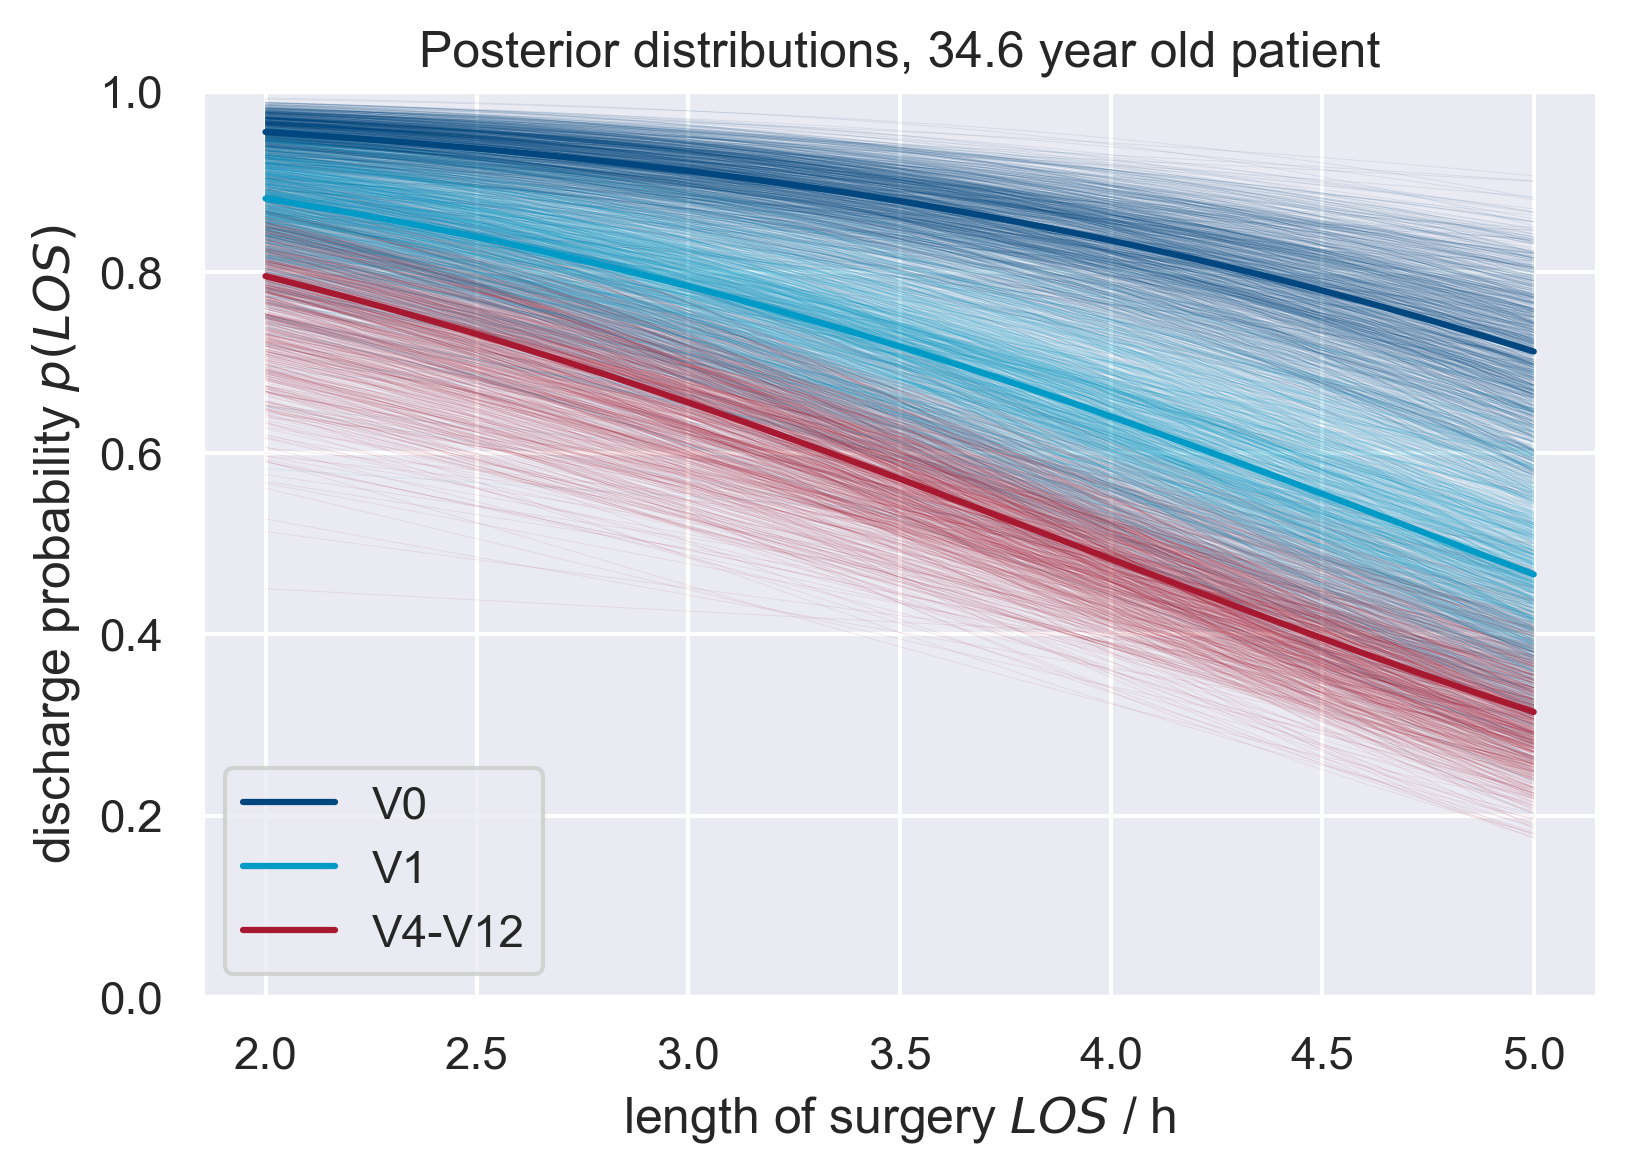
\includegraphics[width=0.5\textwidth]{images/DS19fk1_c0__p_LoS__model_B__traces_V0_V4-12__age_mean.png}&
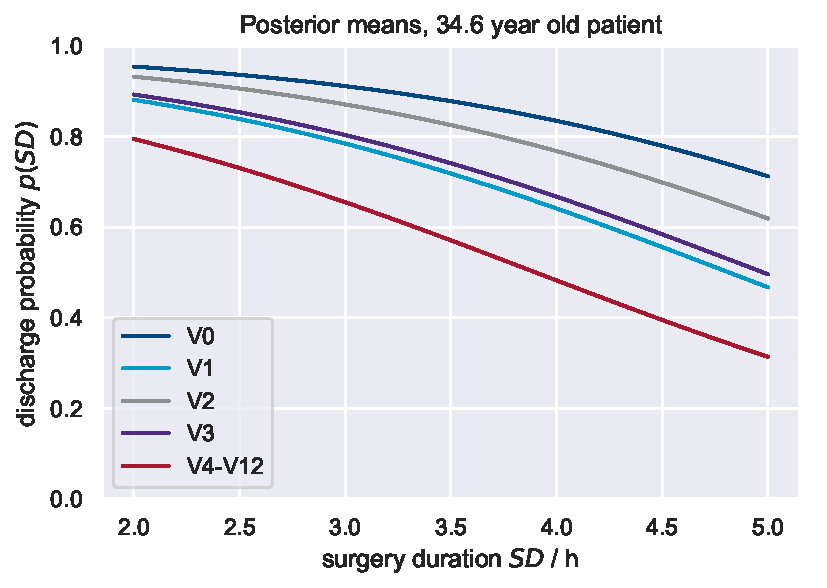
\includegraphics[width=0.5\textwidth]{images/DS19fk1_c0__p_LoS__model_B__mean__age_mean.pdf}\\
(c) & (d) \\
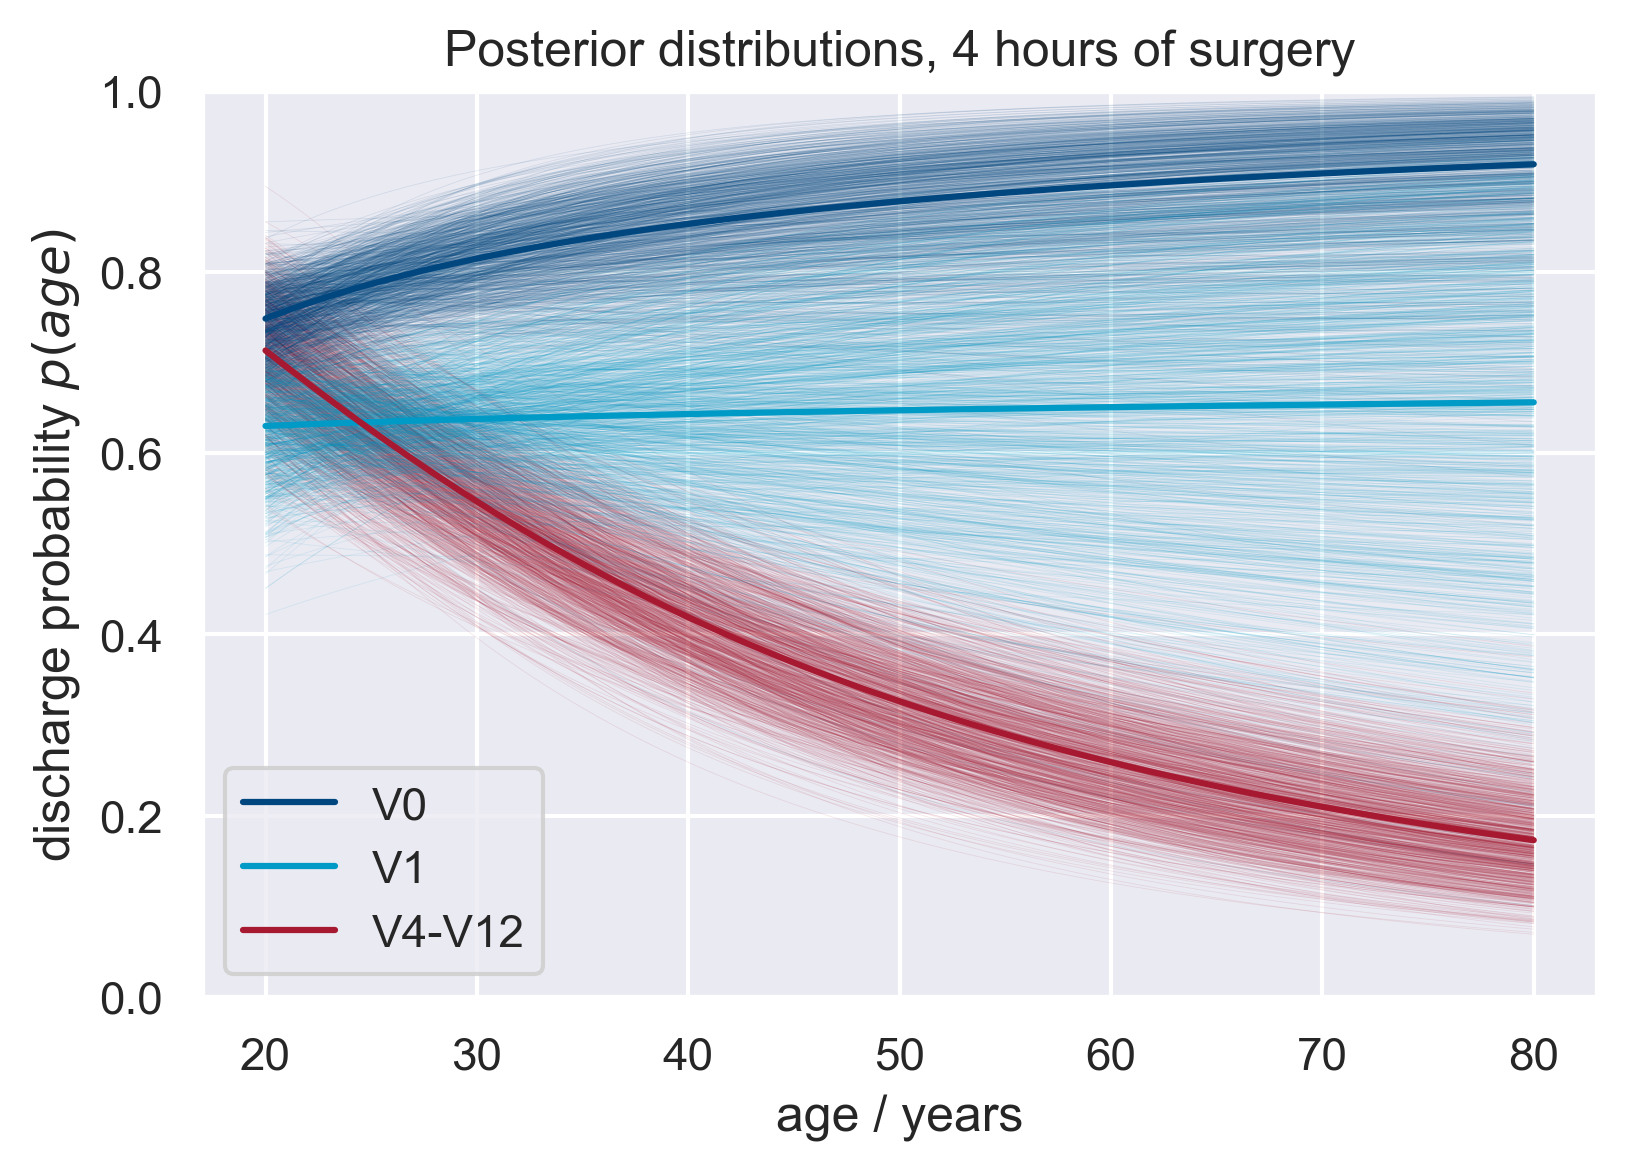
\includegraphics[width=0.5\textwidth]{images/DS19fk1_c0__p_age__model_B__traces__LoS_4h.png}&
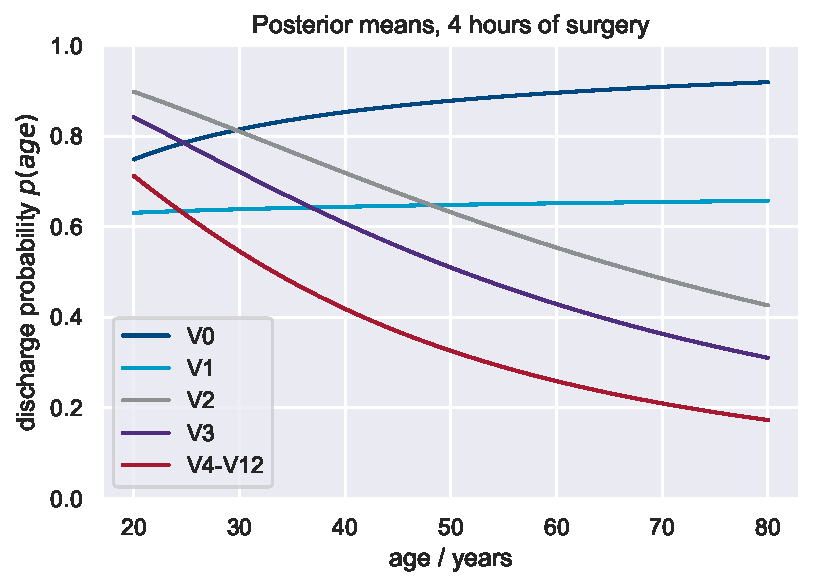
\includegraphics[width=0.5\textwidth]{images/DS19fk1_c0__p_age__model_B__mean__LoS_4h.pdf}\\
\end{tabular}
    \caption{Caption}
    \label{fig:posterior}
\end{figure}

This is visualized in Fig.~\ref{fig:posterior}, which shows the posterior distributions of daily discharge probability $p_i$ as function of LOS (Fig.~\ref{fig:posterior}(a)) and age (Fig.~\ref{fig:posterior}(c)). While the discharge probability decreases with increasing LOS for all pathway variants (Fig.~\ref{fig:posterior}(b)), the effect is different for age. 
The daily discharge probability $p_i$ decreases for Variants V2, V3, and V4-V12 with increasing age of the patients, while its expectation value is constant for $V1$ and even increases by nearly 10\% for V0. Note, that the corresponding graphics for model A \eqref{modelA}, which are not shown here, resemble nearly the same correlations. 
From the clinical perspective, the difference effect of age with respect to the pathway variants might be related to the fact that the most often pathway variants V0 and V1 are only found for older patients of all ages, for whom no complications are expected. 
However, the uncertainty of daily discharge probabilities for V1 is significantly larger compared to V0.

%\subsection{Cholecystitis Pathway Variants}
This section shows the cholecystitis pathway variant plot auto-generated by ProM. Cholecystitis pathway variants are analyzed without activities from the `antibiotics' sub-process and the `monitoring labs' sub-process (see section 3.7 for the activities from the two sub-processes). Clinicians confirmed that these sub-processes are standard monitoring and maintenance systems while the patient is waiting for further diagnosis. Only analyzing activities from the primary cholecystitis pathway significantly reduces the level of clinical variation between patient traces.

The cholecystitis pathway model consists of 10 pathway variants. The 10 pathway variants from the cholecystitis pathway model are shown in Fig.~\ref{fig:cholecystitis pathway variants}, and the number of patient traces that follow each pathway variant are listed in Table \ref{table:cholecystitis variant table}. Pathway variants from Fig.~\ref{fig:cholecystitis pathway variants} are ordered from the most frequent (index 0) to the least frequent (index 9). The most frequent pathway variant (index 0) consists of anesthesia, surgery, and surgical pathology lab. The second pathway variant (index 1) includes surgery without anesthesia because of faulty clinical data.

\begin{figure}[t]
\hspace{-2cm}
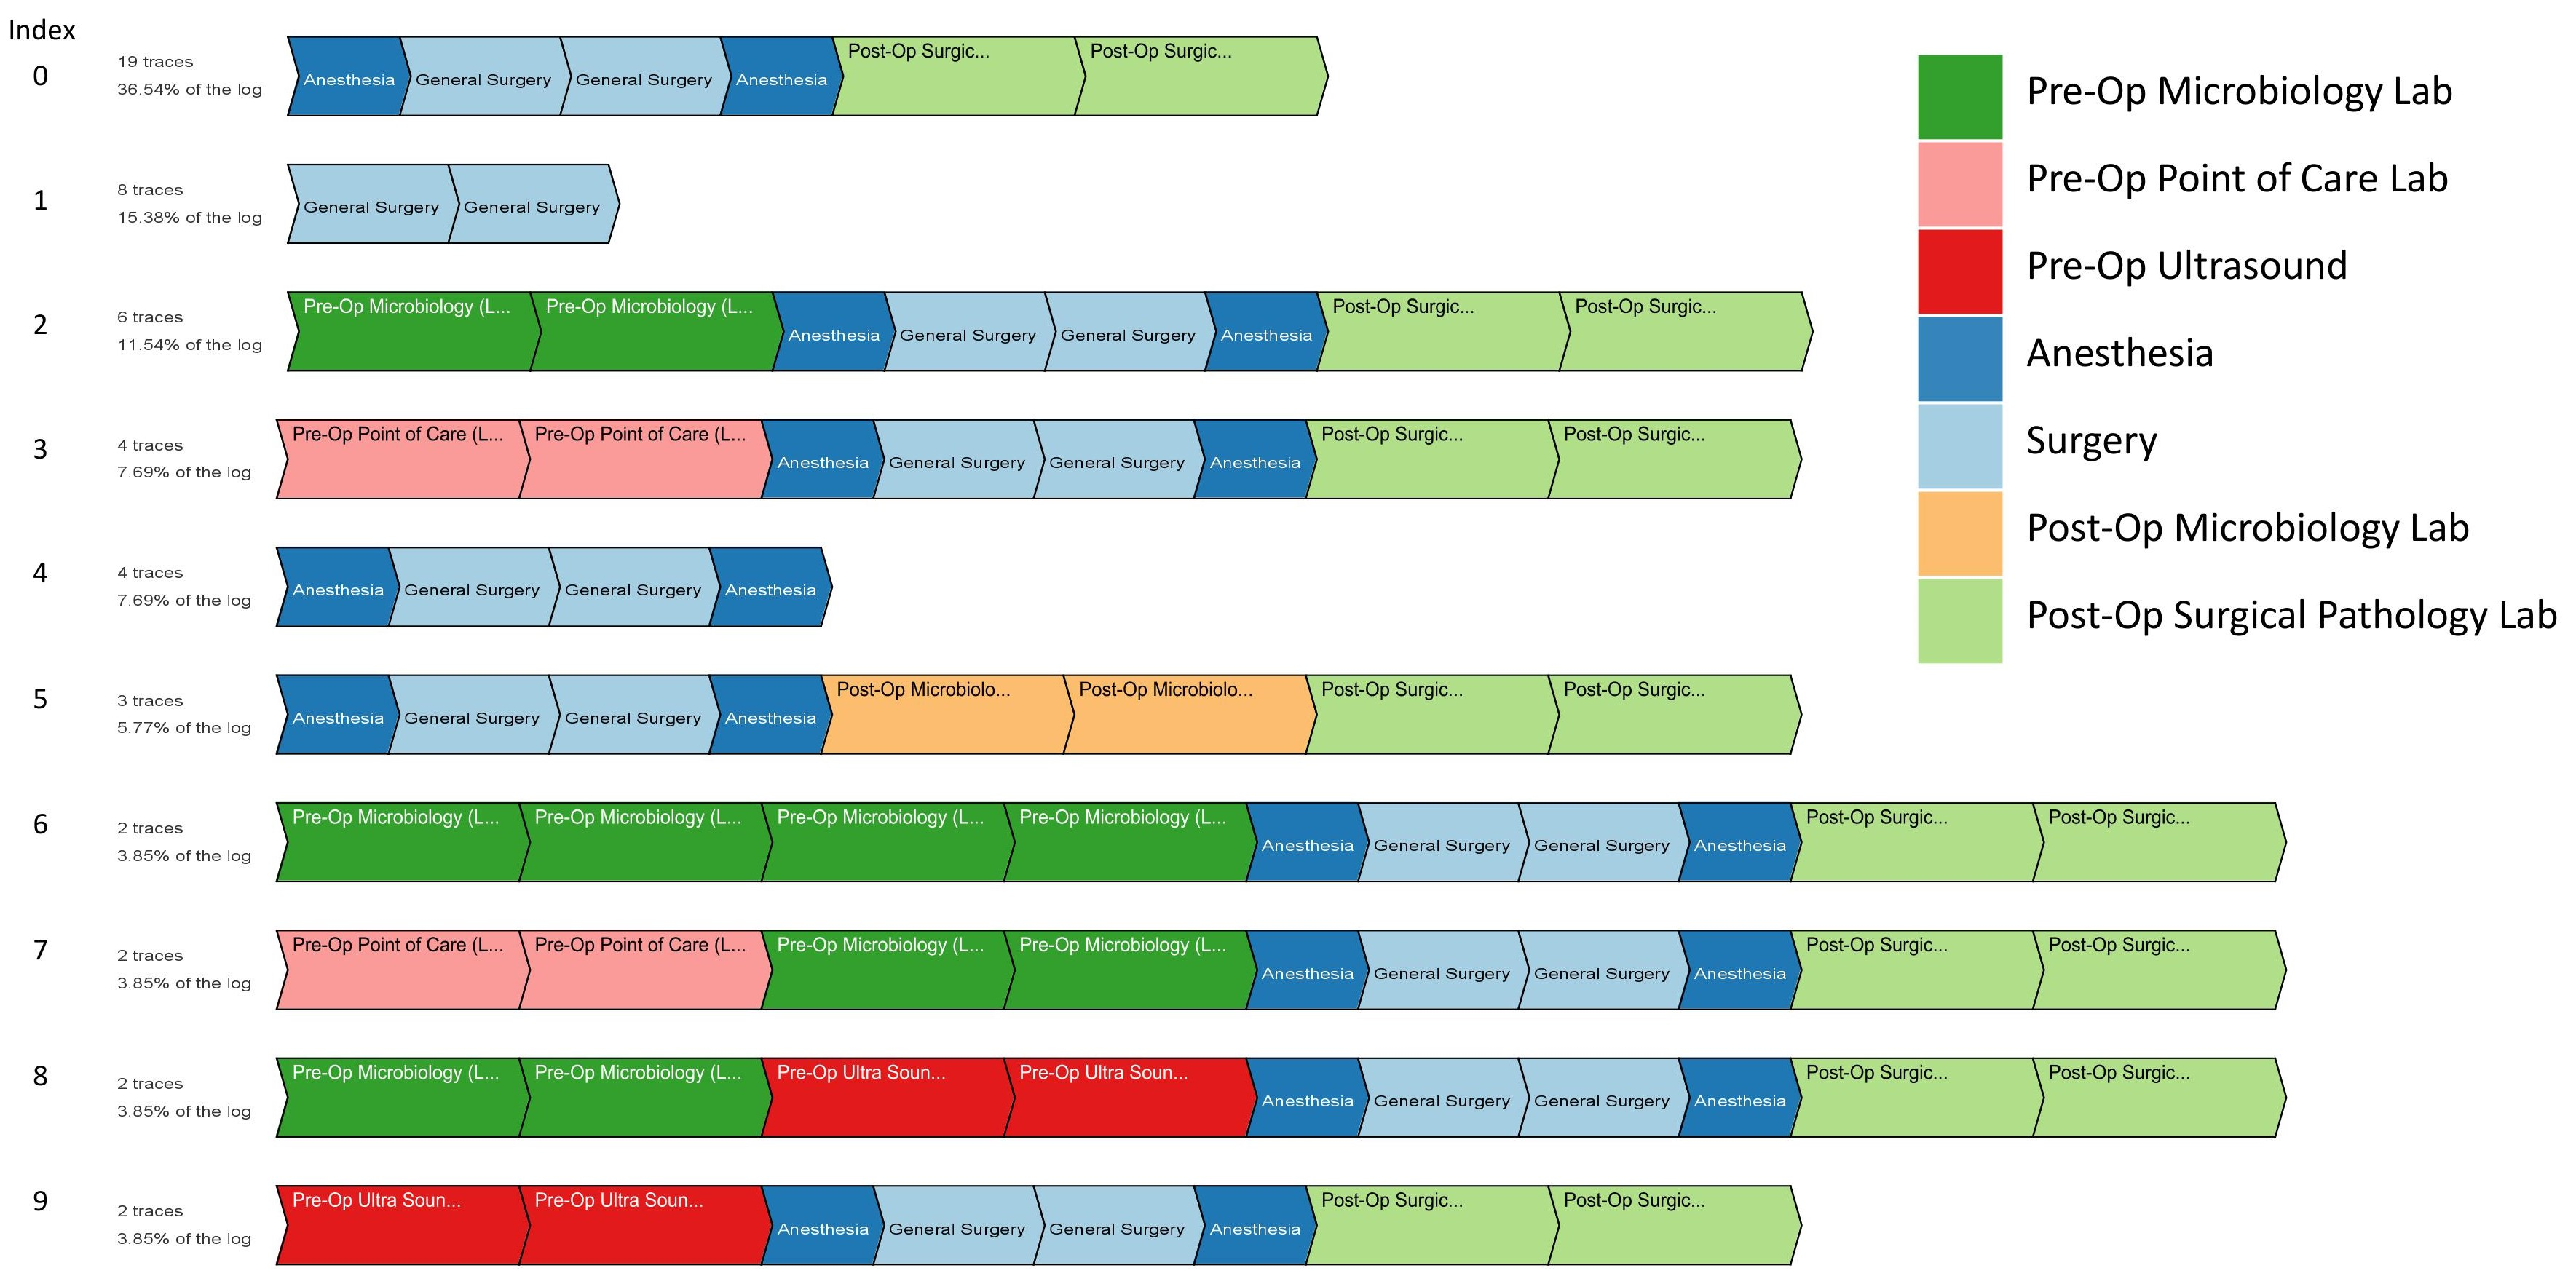
\includegraphics[width=1.5\textwidth]{images/cholecystitis_variant_index_anes.jpg}
\caption{Cholecystitis pathway variants auto-generated by ProM and appended with a legend. The top three pathway variants account for approximately 63\% of the patient traces. The statistics on the left are not readable in this reproduction but are listed in Table \ref{table:cholecystitis variant table}.}
\label{fig:cholecystitis pathway variants}
\end{figure}

\begin{table}[t]
\centering
\caption{Number of patient traces that follow each cholecystitis pathway variant.}
\label{table:cholecystitis variant table}
\begin{tabular}{ l l l }
 \hline
 Index & Number of Patient Traces & Percentage of Patients \% \\ 
 \hline
 0 & 19 & 36.54\\ 
 \hline
 1 & 8 & 15.38\\ 
 \hline
 2 & 6 & 11.54\\ 
 \hline
 3 & 4 & 7.69\\ 
 \hline
 4 & 4 & 7.69\\ 
 \hline
 5 & 3 & 5.77\\ 
 \hline
 6 & 2 & 3.85\\ 
 \hline
 7 & 2 & 3.85\\ 
 \hline
 8 & 2 & 3.85\\ 
 \hline
 9 & 2 & 3.85\\ 
 \hline
\end{tabular}
\end{table}

\subsection{Cholecystitis Pathway Model}
The cholecystitis pathway model visualized by \texttt{`Inductive Visual Miner'} incorporates activities from the `antibiotics' sub-process and the `monitoring labs' sub-process. A breakdown of the reformulated cholecystitis pathway model into one primary pathway and two concurrent sub-processes is shown in Fig.~\ref{fig:cholecystitis pathway model}, and the model notations are summarized in Table \ref{table:notation table}. The first pathway model in Fig.~\ref{fig:cholecystitis pathway model} is the primary pathway, followed by the `antibiotics’ sub-process and the `monitoring labs’ sub-process. Patient traces can execute any combination of the two sub-processes concurrently with the primary pathway. The eight patient traces that follow the second pathway variant (index 1) do not conform to this pathway model because of faulty clinical data. Based on this model, pre-operation haematology and chemistry labs tend to span the entire pre-operation process, while pre-operation antibiotics are taken closer to surgery.

\begin{figure}[t]
\centering
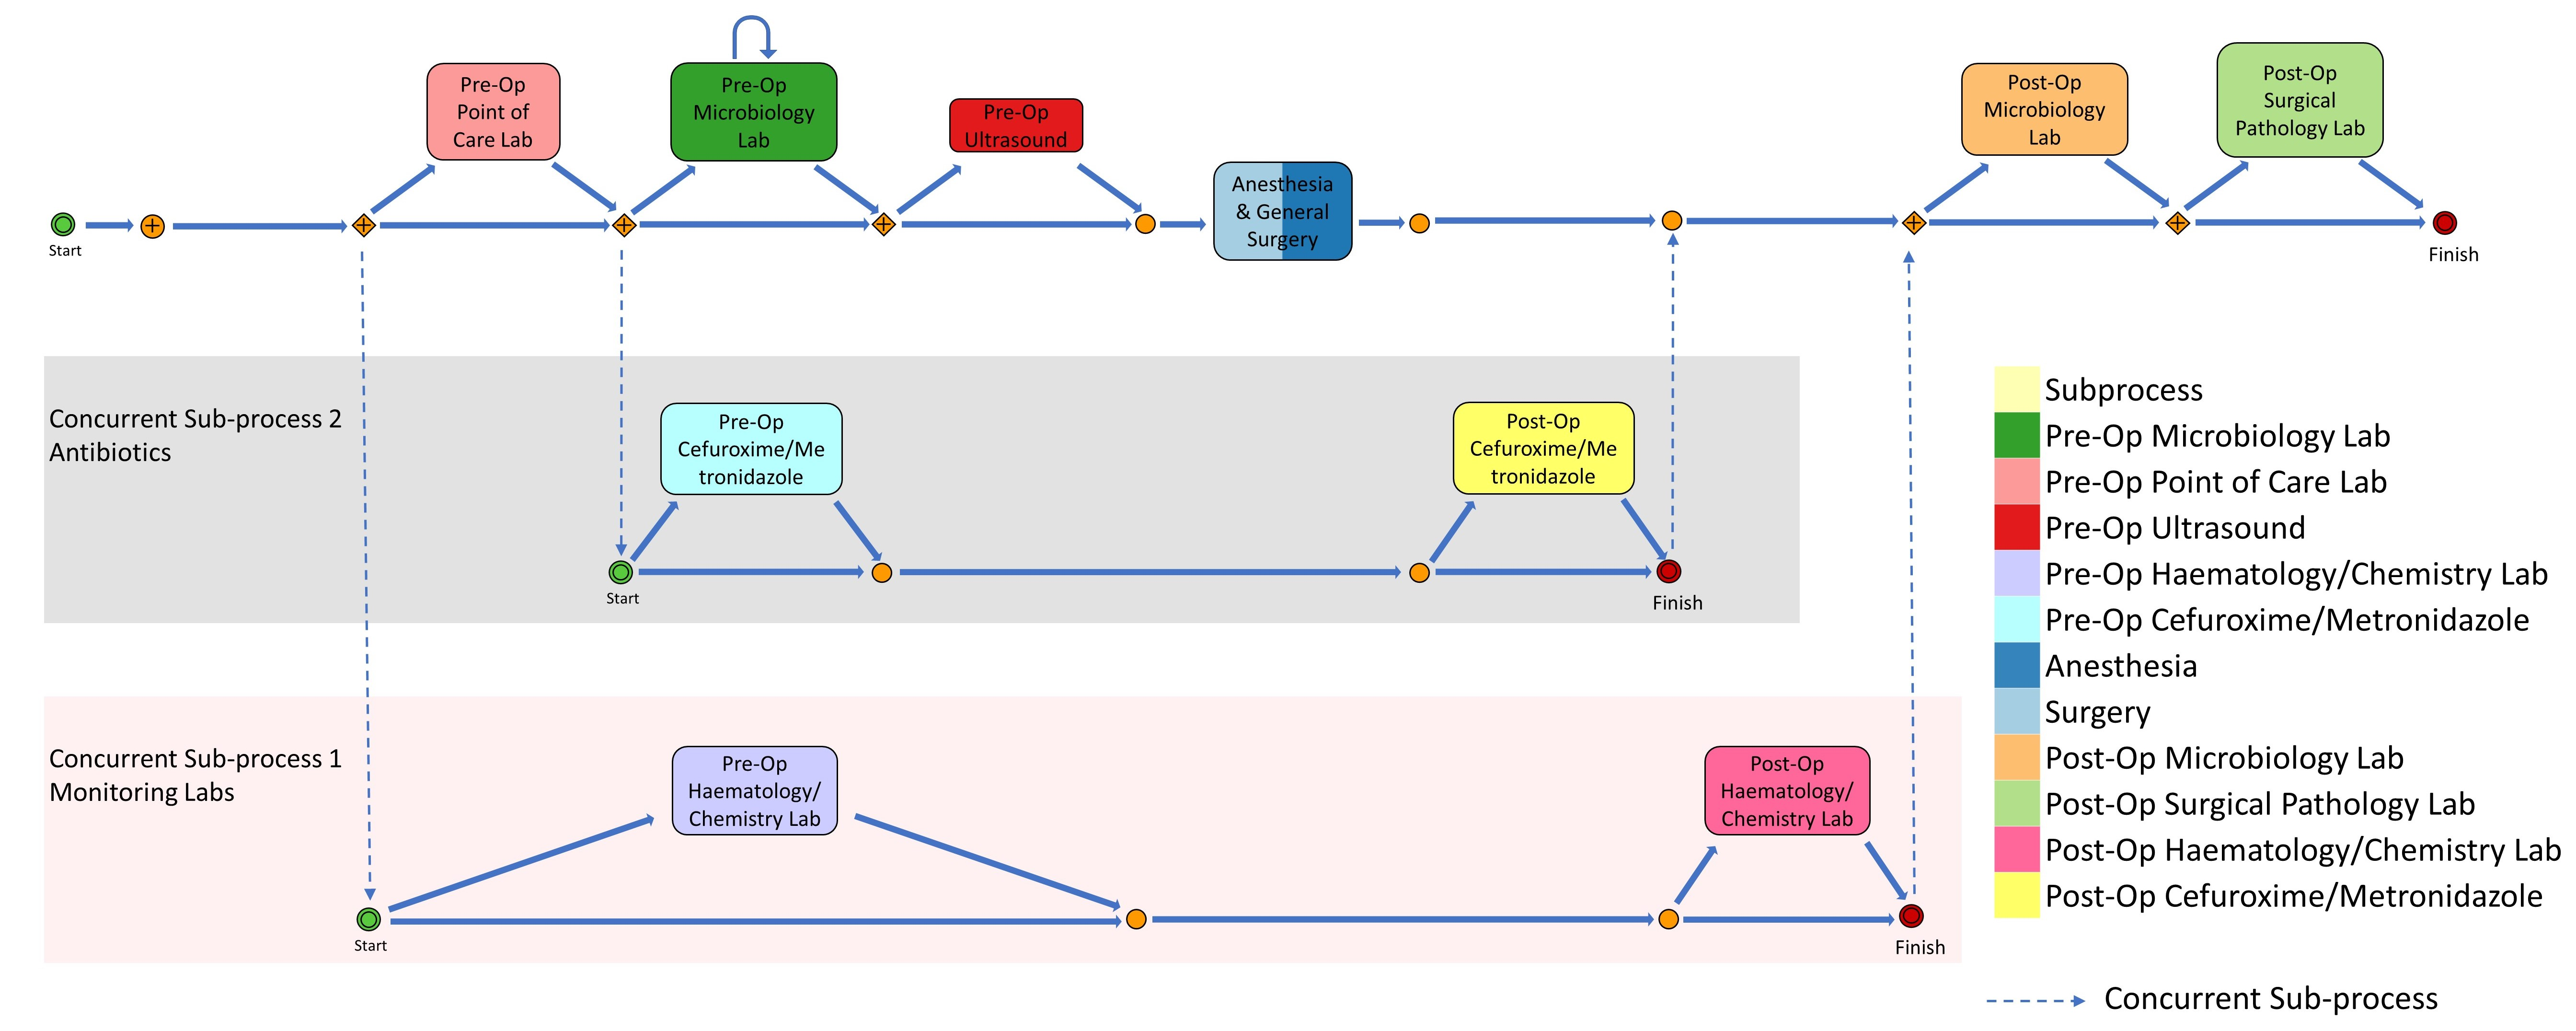
\includegraphics[width=18cm,angle=270]{images/communicative_cholecystitis_process_models_anes.jpg}
\caption{Cholecystitis pathway model. The model is broken down into one primary pathway and two sub-processes.}
\label{fig:cholecystitis pathway model}
\end{figure}

\section{Conclusion}
Healthcare pathways are critical for maintaining quality of care and improving health outcome for all patients, but there is no consensus on a healthcare pathway mining pipeline suitable for hospital implementation that supports pathway discovery from hospital health records. Business process modelling methods are used to design a process mining pipeline that produces concise and comprehensible healthcare pathway models from hospital records, and supports conformance analysis and enrichment of the discovered pathways. The proposed process mining pipeline successfully constructs concise pathway models for the appendicitis and cholecystitis case studies. The produced healthcare pathway models are easy for clinical interpretation and provide an unbiased overview of real patient traces through the treatment process. Preliminary analysis on building a machine learning model to predict post-operation length of stay, using information extracted by the process mining pipeline, is showing promising results. This means that the proposed mining pipeline has the potential to support the development of machine learning models to further relate healthcare pathways to performance indicators. This study has established the use of business process modelling methods for the improvement of healthcare pathway mining methods, and there is value in investigating the capabilities of other business process modelling tools for healthcare pathway mining purposes.

\begin{table}[h]
\centering
\begin{tabular}{p{11cm}} 
 Summary points\\ 
 What was already known:
 \begin{itemize}
     \item Healthcare pathways are critical for reducing clinical variability, affecting operational excellence, and thereby maximizing health outcomes.
     \item  Most healthcare pathways result from clinician-led practice rather than explicit pathway design via a consensus model and systems approach. 
     \item  There is currently no consensus on a systematic healthcare pathway mining method that supports explicit design and conformance analysis of concise and comprehensible healthcare pathway models.
 \end{itemize}
 What this study adds:
 \begin{itemize}
     \item  The use of business process modelling methods improves the automatic mapping of healthcare pathways from clinical data.
     \item The application of business process modelling methods to healthcare pathway enables deviations from typical treatment pathways to be identified; and predictions for future treatment duration to be made, all using standard clinical data timestamps. 
 \end{itemize}
\end{tabular}
\end{table}
